\pagebreak
\section{AR Annotation using 3D sensors}
\label{sec:3D}

A second example of the interaction dimension of the Social AR Continuum is in interaction with 3D depth data. The AR annotation can be placed in a 2D plane (lower fidelity) or on a 3D depth registration (higher fidelity), which then can be mapped into social proximity. 

This section describes a wearable system that allows people to place and interact with 3D AR annotations placed around them (\cite{Nassani2015a, Nassani2015}, Figure \ref{fig:mgia15:teaser}). It uses two wearable technologies: a head-worn wearable computer (Google Glass\footnote{https://en.wikipedia.org/wiki/Google\_Glass}) and a chest-worn depth sensor (Google Tango \footnote{https://en.wikipedia.org/wiki/Tango\_(platform)}). Google Glass is used to generate and display virtual information to the user, while the Tango is used to provide robust indoor position tracking for the Glass. The Tango enables spatial awareness of the surrounding world using various motion sensors including 3D depth sensing, an accelerometer and a motion-tracking camera. Using these systems together allows users to create an AR annotation via voice input and then register this annotation to a physical object or position in 3D space as an augmented annotation. This work describes the design and implementation of the system, user feedback, research implications, and directions for future work.  

\begin{figure}[ht]
  \centering
  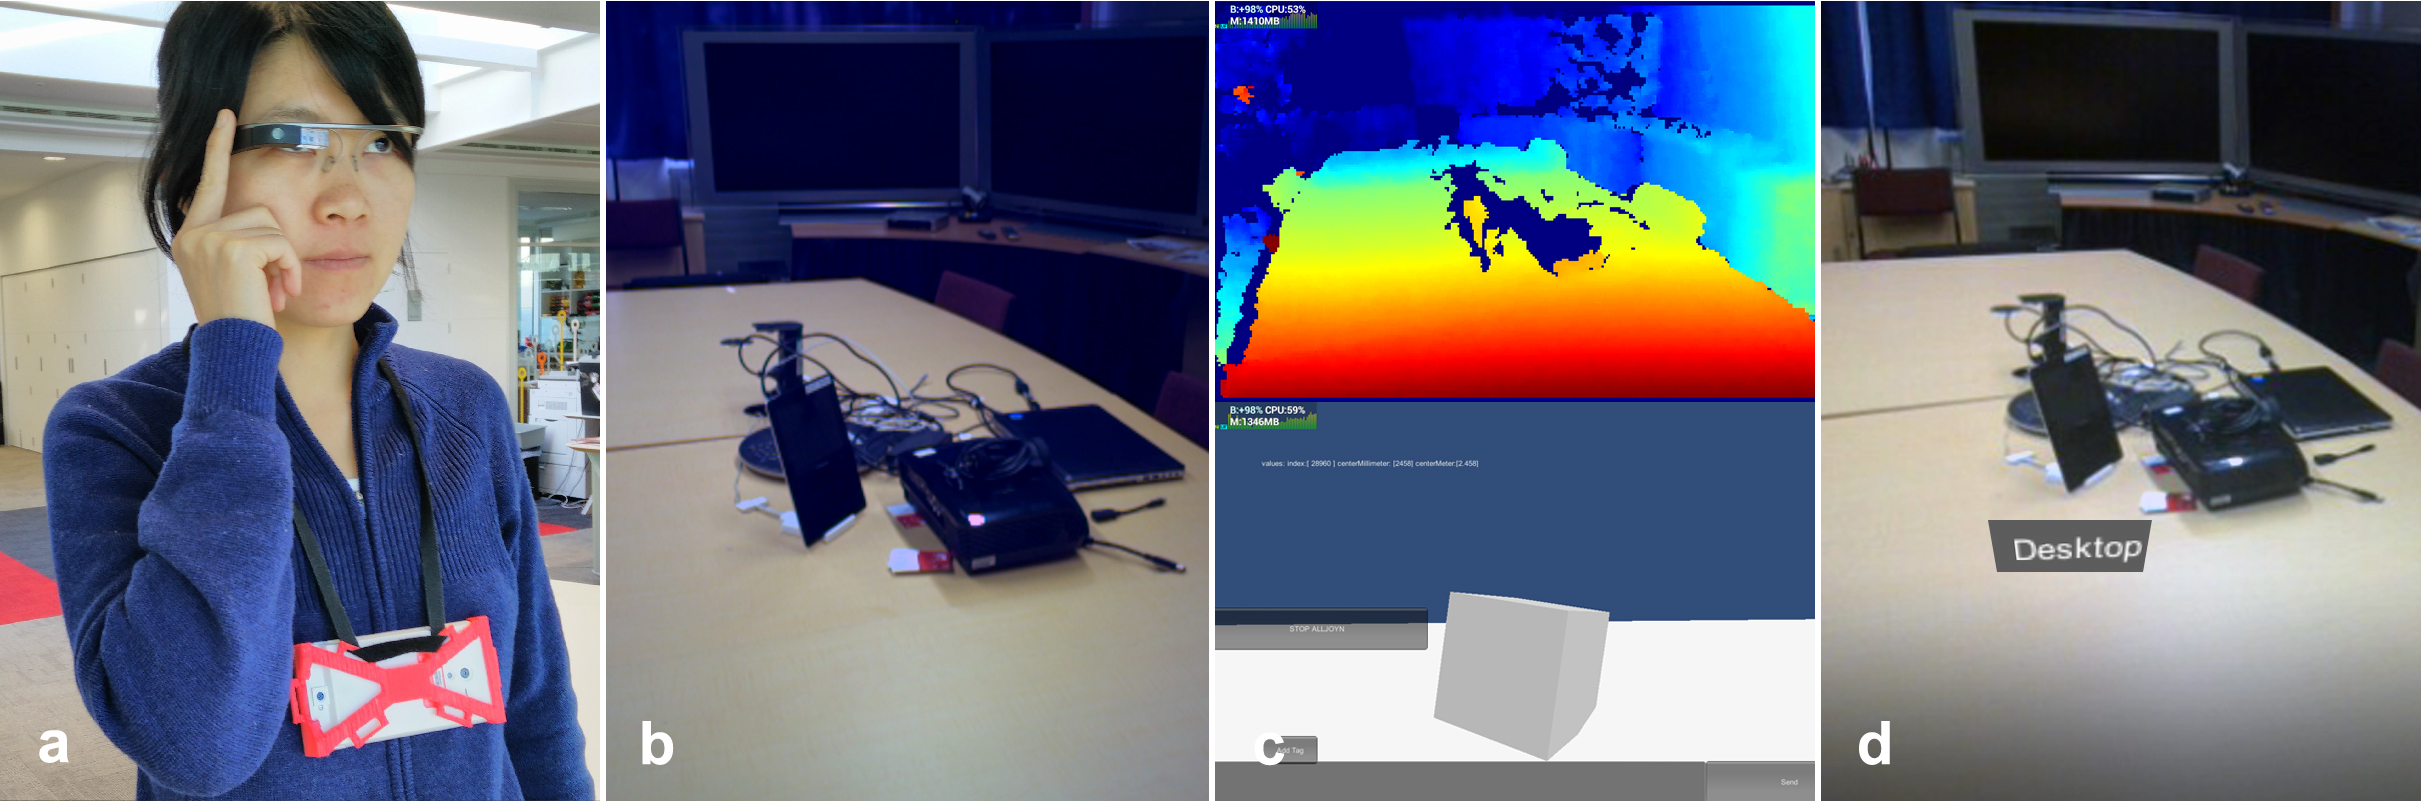
\includegraphics[width=\linewidth]{images/62-3d-mgia15/sampleteaser-01.jpg}
  \caption{AR annotation application scenario. (a) The setup; (b) A sample indoor environment; (c) The depth data from the Tango sensors; (d) The AR view through the Glass display.}
  \label{fig:mgia15:teaser}
\end{figure}

This system combines multiple wearable technologies through a wireless network. The system is small and light enough to be comfortably worn, allowing for mobility in the physical world, and being available for annotation not only on 2D surfaces also in 3D space. For example, if the user walks closer to or away from the AR annotation (e.g., 3D text or models), it will appear larger or smaller according to the changes in the perspective view. The system combines Google Glass and Google Tango together to provide a compelling wearable AR experience. Google Tango is a self-contained hand-held device that uses a motion-tracking camera, 3D depth sensing, a nine-axis accelerometer, gyroscope and compass sensors. It has a rear-facing 4MP RGB/infrared camera, a 180-degree field-of-view fisheye rear-facing camera, a 120-degree field-of-view front-facing camera, and a 320 x 180 depth sensor. In contrast, Google Glass has no depth-sensing capability but combines computing and display in a highly compact form factor. 

% Connecting the two devices enables us to prototype future wearable AR interfaces such as what might be possible with Microsoft Hololens\footnote{https://www.microsoft.com/microsoft-hololens/en-us} or other devices.


\subsection{System Design}

The main application scenario for our prototype system is around sharing messages through creating and viewing location-based AR annotations registered in a small scale physical environment. The user wearing the system walks into a room and then places AR annotations at various places or on objects offline (asynchronously) so that the AR annotation can be viewed later by the same user or by a different user. The AR annotation content is created by using voice input and placed where the user is looking. The distance between the AR annotation and the user is between 0.5 to 4 meters (according to Google Tango depth camera specifications) The AR annotations can be meaningful for users, for example, reminding them of something interesting in this space, or sharing the message with other users as a collaborative tool. The system should work in an arbitrary unprepared indoor environment where no previous knowledge about the space is required. 

Traditionally AR annotation tracking uses two different approaches at different ends of the technology spectrum (see Figure~\ref{fig:mgia15:spectrum}) based on the level of detailed information required. At one end, there is GPS location-based tracking that can be implemented in a light-weight HMD such as Glass. On the other end, 3D depth-sensing cameras incorporated into a hand-held device (HHD) are capable of indoor tracking and localisation. The aim of this system is to combine the benefits of a light-weight HMD with self-contained mobile 3D depth tracking, offering not only the outdoor GPS based tracking but also vision-based indoor tracking for AR annotation applications. 

\begin{figure}[ht]
  \centering
  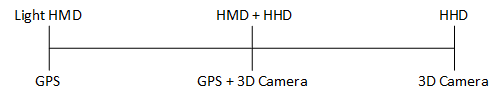
\includegraphics[width=0.8\linewidth]{images/62-3d-mgia15/tango_paper_continuum.png}
  \caption{The spectrum of AR annotation tracking. A head-mounted display with GPS is ideal for outdoor tracking. Hand-held devices (3D camera) can be used for indoor tracking. Glass+Tango enables indoor AR annotation tracking on a light HMD.}
  \label{fig:mgia15:spectrum}
\end{figure}

\subsection{Implementation}

The system consists of two wearable devices, a Google Glass HMD and a Google Tango chest-mounted 3D depth and sensor (see Figure~\ref{fig:mgia15:framework}). The two devices communicate with each other wirelessly. The Tango extends Glass' sensing ability by sharing the location and pose of the user as well as the annotated target position in the real world. The Glass dynamically overlays an AR annotation based on the spatial information received from the Tango, and the background of the Glass display is set to black to act as an optical see-through display (see Figure~\ref{fig:mgia15:ui}). A white square is displayed on the Glass screen to indicate the centre point at which the tango depth camera is facing. The user can initiate the wireless connection by using a three-finger touch gesture on the Glass touchpad, and the AllJoyn\footnote{https://en.wikipedia.org/wiki/AllJoyn} library is used for networking.

\begin{figure}[ht]
  \centering
  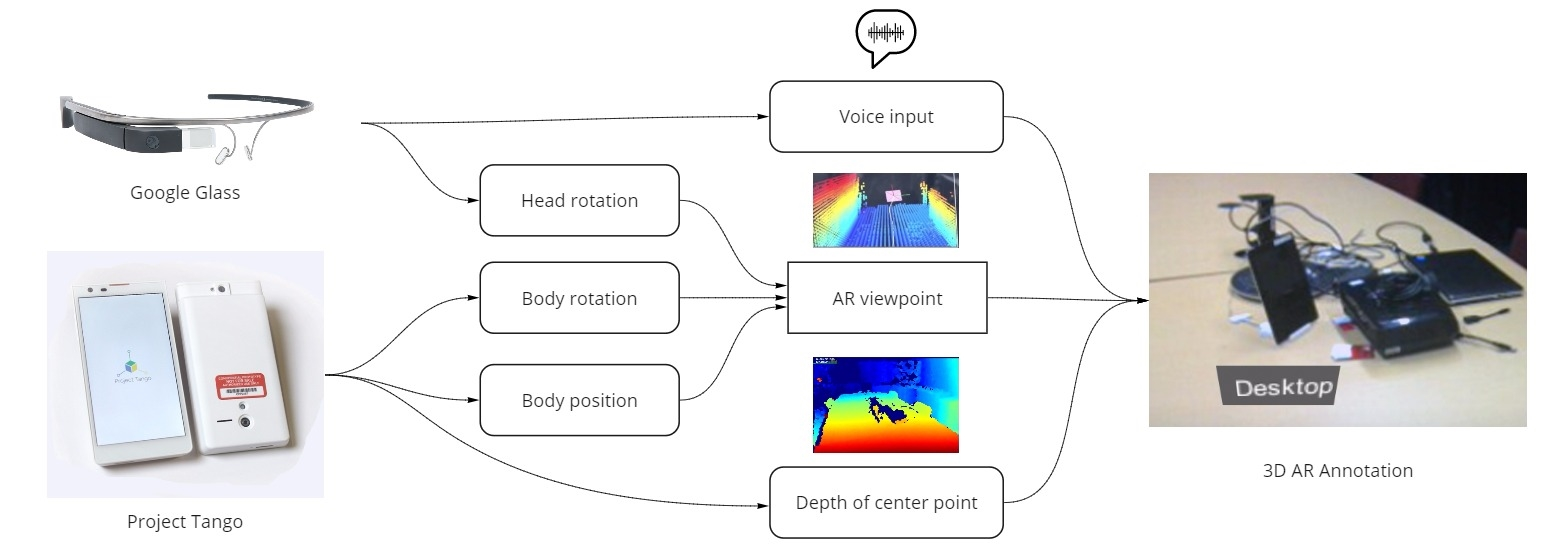
\includegraphics[width=\linewidth]{images/62-3d-mgia15/mgia2015-system.jpg}
  \caption{System workflow of AR Annotation using 3D sensors. Google Glass detects user voice input for the annotation text content. The AR viewpoint is calculated based on the head rotation from Google Glass, body rotation and position from Google Tango. Google Tango also provides the depth (z-axis) for where to place the annotation on top of the real world.}
  \label{fig:mgia15:framework}
\end{figure}

Once the system starts on the Tango, it creates a reference coordinate of the surrounding environment. When the user moves, the motion sensor on the Tango will detect the body position and rotation from the reference origin, both of which are then wirelessly transmitted to the Glass. Combing the head rotation detected by the sensors on the Glass, the AR Viewpoint position can be calculated. The position of the AR viewpoint is calculated by adding a measured distance in height from Tango's position to adjust for the height difference between the Glass and Tango. The orientation of the AR viewpoint mainly depends on the body's rotation but will be adjusted with the head and body pose difference, if the user turns their head towards a different direction from their chest. 

A speech recognition service is running in the background on the Glass to detect the users' voice input and convert it into a short-word text. The text will appear on the upper-left corner of the display for the user's confirmation (see Figure~\ref{fig:mgia15:ui}). The upper-left corner shows the last words captured via the voice recognition service, and a white square indicates the centre position of Tango's RGB depth frame. The text in the middle of the display "Cup" is an AR annotation overlaid on top of a physical cup. This function is implemented as an Android service that utilises the Google API for speech recognition\footnote{https://developers.google.com/glass/develop/gdk/voice}, and so requires an internet connection. Once the user is satisfied with the recognised text, they can tap on the Glass touchpad while looking where they wish to add the AR annotation by using the white square in the display. The Glass sends a request to Tango to identify the location of the AR annotation in 3D space.

\begin{figure}
  \centering
  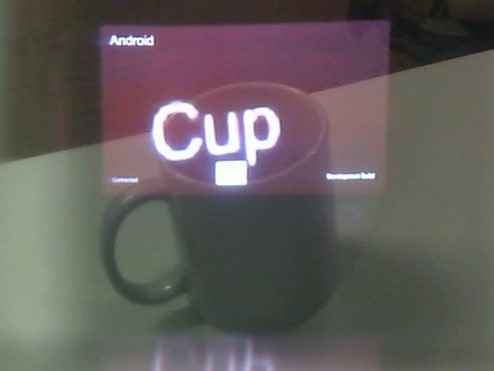
\includegraphics[width=0.6\linewidth]{images/62-3d-mgia15/WIN_20150614_204531_2.jpg}
  \caption{View through Glass display of a cup overlaid with an AR annotation.}
  \label{fig:mgia15:ui}
\end{figure}

Combining the AR viewpoint and the recognised text, the target position could be converted (the centre point of the depth image indicated by the white square) to the global position relative to the origin. The Tango returns the global position of the AR annotation to the Glass. This information is used to construct an AR annotation with the speech recognised text that is overlaid on the top of the Glass camera view.

\subsection{User Study}

A user study was conducted (see Figure~\ref{fig:mgia15:scenario}) with ten participants, four female, six male, ranging in age between 23 to 33 years old ($SD= 4.35$). The main focus of the study was to measure the usefulness of the proposed system. Participants were asked to create three different AR annotations for three different objects inside the room, with voice input, and then to walk around to observe how well the AR annotation was placed at the selected location. Participants had the freedom to assign a text using voice input to an object they wished in the test. The experimenter explained the task before the experiment and gave examples of target objects and names to use for voice input. All participants completed the task within five minutes. 

\begin{figure}
  \centering
  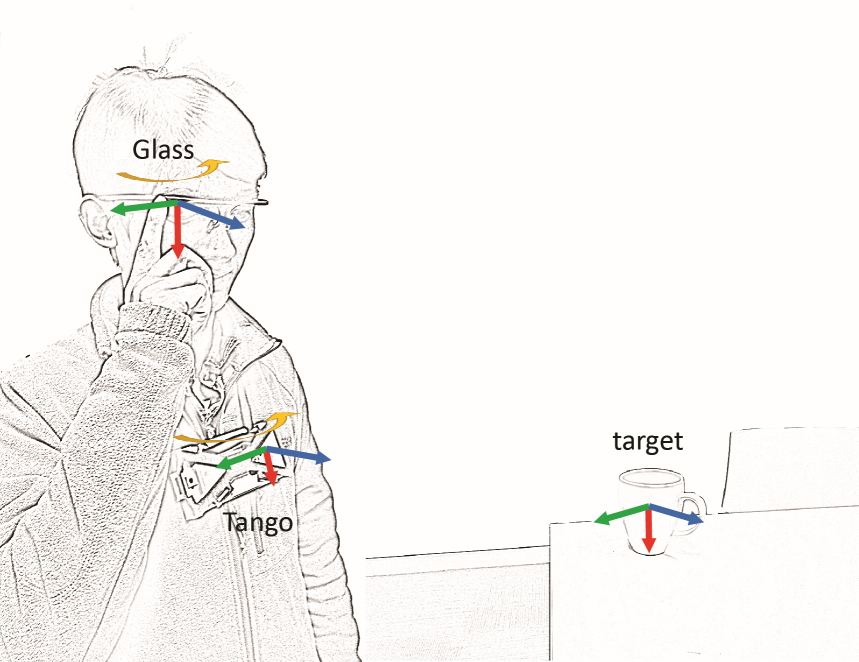
\includegraphics[width=0.6\linewidth]{images/62-3d-mgia15/axis_lo_small.jpg}
  \caption{User study scenario}
  \label{fig:mgia15:scenario}
\end{figure}

Qualitative feedback about the system was collected from participants, including how they would describe their experience using our system, what they liked and disliked. The same set of questions (Table \ref{table:mgia15:questions}) were asked in four categories: (C1) Using the voice commands to create an AR annotation, (C2) Tap on glass touch panel to attach the AR annotation, (C3)  Walk around to find an AR annotation stuck to the original position, (C4) Overall AR annotation experience.

\begin{table}
  \centering
    \caption{Survey questions}
    \label{table:mgia15:questions}
    \begin{tabular}{r l}
    \hline
    Q1 & I found it easy to use \\ \hline
    Q2 & I found it natural to use \\ \hline
    Q3 & I found it physically challenging \\ \hline
    Q4 & I found it mentally challenging \\ \hline
    Q5 & I found it useful \\ \hline
    \end{tabular}
\end{table}

\subsection{Results}

The answers were captured on a Likert scale of 1 to 7 in which 1 = "strongly disagree", and 7 = "strongly agree". The One-sample Wilcoxon Signed-Rank test was used on the results to measure significance. Based on the results, the results found that participants rated significantly higher than neutral (4) on Q3 ($p=0.01, 0.009, 0.007, 0.041$) and Q4 ($p=0.014, 0.009, 0.007, 0.01$) for all categories (C1, C2, C3, C4). Q2 ($p=0.033$) and Q5 ($p=0.015$) were rated significantly higher for category (C3). Q1 for C4 was rated significantly higher ($p=0.014$) (see Figure~\ref{survey_results}). The results for other tasks were rated less significant than neutral level (4). Participants rated the task of walking around the environment as useful with an average score of 5.2 out of 7, as well as being not mentally challenging with an average score of 2 out of 7. This highlights the usefulness of the system in assigning AR annotations and recognising them when they appear on their display while walking around the environment. 

\begin{figure}[ht]
  \centering
  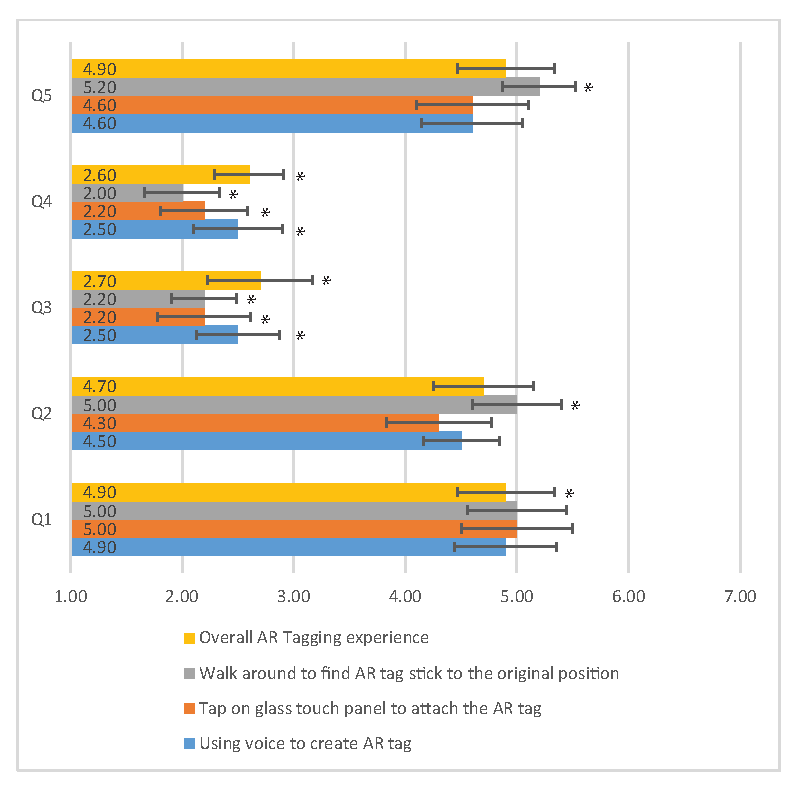
\includegraphics[width=\linewidth]{images/62-3d-mgia15/user_study_results2.eps}
  \caption{Average results of survey questions. Bars indicate standard error. *=statistically significant}
    \label{survey_results}
\end{figure}

In addition to the survey, participants were asked open-ended questions to comment on the system usability. A total of 3 out of 10 participants mentioned that they would use this system for virtual sticky notes, and they also provided some positive feedback such as "\textit{the system could be useful for finding a meeting room or a colleague's desk in an open plan area}". There were also a few suggestions for improving the system, such as "allow the user to manually adjust the location of the AR annotation" or "integrate with eye-tracking to assist placing the AR annotation within the field of view". Participants appreciated the concept of wirelessly connecting depth camera to a wearable HMD to enable the 3D spatial tracking.    

\subsection{Discussion}

While our prototype system demonstrates the concept of harmonising the use of multiple wearable devices for AR visualisation, there are a few limitations in the current implementation of the system. It was observed that some users had difficulties with voice input as they were not native English speakers, which made the participants use several attempts before the intended word was correctly recognised.  

The current system tracks the 3D environment relative to the starting position, which requires users to start the system at the same position and orientation in each test trail to keep the annotation in place between uses for sharing. This could be overcome in the future by storing the reconstructed 3D map of the environment and reusing it instead of generating it from scratch every time. 

% \subsection{Future Application Scenarios}
Many implementation scenarios could benefit from combining a light-weight HMD with a chest-worn 3D depth camera, such as 1) navigation, 2) Remote collaboration and 3) Social sharing. This section describes each of these in more detail.

Navigation is a scenario where this system can be useful. The user could navigate in an outdoor environment using GPS on Glass or similar smart glass display. Google Glass, being an unobtrusive HMD, allows for hands-free navigation. However, when the user enters a building, the GPS stops working, and the system switches to indoor navigation using the 3D depth camera of the Google Tango device. Combining two devices enables a seamless transition during a navigation experience. For example, a person could be shopping to find a particular item and use outdoor GPS tracking to guide them to the store. Once inside the store, the Tango depth-sensing hardware can help with navigating to find a particular product on the shelf.

Remote collaboration is another scenario where this application could be useful. A local user could transmit reconstructed 3D geometry of the environment using the Tango device to the remote user. The remote user will then have a more detailed view of the environment compared to 2D sharing such as with a video stream. With the 3D geometry of the environment, the remote user can view the scene from different angles, which helps provide a better understanding of the surroundings of the local user. Placing AR annotations in a 3D environment helps maintain the location of the AR annotation especially when the viewing perspective is changed to the point from when it was originally recorded.

Additional use of the system could be in a social sharing experience where multiple users of the system could collaborate to add, edit and manipulate AR annotations in the shared environment. Multiple users wearing depth sensors could see the same annotation while they are face-to-face or if they are remote, they can see a live stream from the local user with the AR annotation. Also for asynchronous collaboration, user A can add an annotation to a physical object/location, then user B can come in later (when user A has left) and view and interact with the AR annotation.

The system described in this section was designed and implemented in 2014. In 2019, similar capabilities can be found in a self-contained HMD unit such as HoloLens or Magic Leap. If similar project to be implemented today, the Magic Leap HMD can be used with no additional hardware.


\subsection{Conclusions}

This section presented a wearable AR system combining tracking technologies to provide a compelling indoor AR experience for spatial annotation applications, especially in asynchronous collaboration scenarios where the users of the system are not required to be online at the same time. By wearing the system, users can create AR annotations with text content generated by voice input, and place them where they are looking. The AR annotation can be visualised in place as a reminder for the users.  

